\section{Desafíos Técnicos y Soluciones}

\subsection{Desafíos de Canal y Propagación}

Particularmente llamativo es el hecho de que el canal D2D en entornos NTN presente características radicalmente distintas a las de las redes terrestres convencionales. 

La combinación de gran distancia, movimiento relativo extremo y efectos atmosféricos genera pérdidas de propagación severas, desvanecimiento por sombra y variaciones rápidas de fase. Trabajos recientes en arquitecturas LEO para D2D destacan que el Doppler severo y la alta variabilidad del canal constituyen los principales obstáculos para enlaces estables \cite{DeGaudenzi2026_NTN}. 

Análisis de cobertura en escenarios reales refuerzan estas observaciones, mostrando que la disponibilidad de servicio cae drásticamente en entornos urbanos con obstrucciones o en latitudes altas \cite{Ullah2026_D2D}. La arquitectura propuesta incorpora estimación avanzada de canal asistida por IA y beamforming dinámico para mitigar estos efectos, aunque no los elimina por completo.

\subsection{Movilidad y Handover}

Uno de los desafíos persistentes al desplegar conectividad D2D en constelaciones LEO radica en la gestión eficiente de handover frecuente. 

A diferencia de las redes terrestres, donde los usuarios se mueven frente a infraestructuras fijas, aquí es la infraestructura la que se desplaza a gran velocidad respecto al usuario. Esto genera ventanas de visibilidad cortas y exige mecanismos de predicción de trayectoria y preparación anticipada de enlaces. Las técnicas de mitigación Doppler y timing advance avanzadas de 3GPP Rel-19 ayudan, pero resultan insuficientes en escenarios de alta densidad o movilidad combinada (usuario + satélite).

La solución propuesta incluye un protocolo de handover predictivo TN-NTN que aprovecha gemelos digitales para minimizar interrupciones y optimizar el timing de conmutación.

\subsection{Eficiencia Energética y Escalabilidad}

Lejos de ser un asunto resuelto, la eficiencia energética se convierte en un cuello de botella crítico cuando se pretende conectar miles de millones de dispositivos mediante NTN. 

El uplink satelital exige mayor potencia de transmisión desde el dispositivo, impactando directamente la autonomía de baterías en terminales IoT y smartphones. Revisiones comprehensivas del campo 6G señalan que la escalabilidad masiva solo será viable si se logra una orquestación inteligente que minimice el consumo mediante selección dinámica de enlaces y modos de transmisión de baja potencia \cite{Wang2025_NTN6G}.

\begin{table}[t]
\centering
\caption{Trade-offs arquitectónicos en convergencia D2D-NTN}
\label{tab:tradeoffs}
\begin{tabular}{lcc}
\hline
Aspecto & Ventaja & Desventaja Principal \\
\hline
Cobertura & Global y resiliente & Alto consumo energético uplink \\
Latencia & Aceptable con payloads regenerativos & Mayor que TN puro \\
Escalabilidad & Alta con orquestación & Complejidad de gestión \\
Interferencia & Gestionable con beamforming & Desafiante en bandas compartidas \\
\hline
\end{tabular}
\end{table}

\begin{figure}[t]
\centering
% 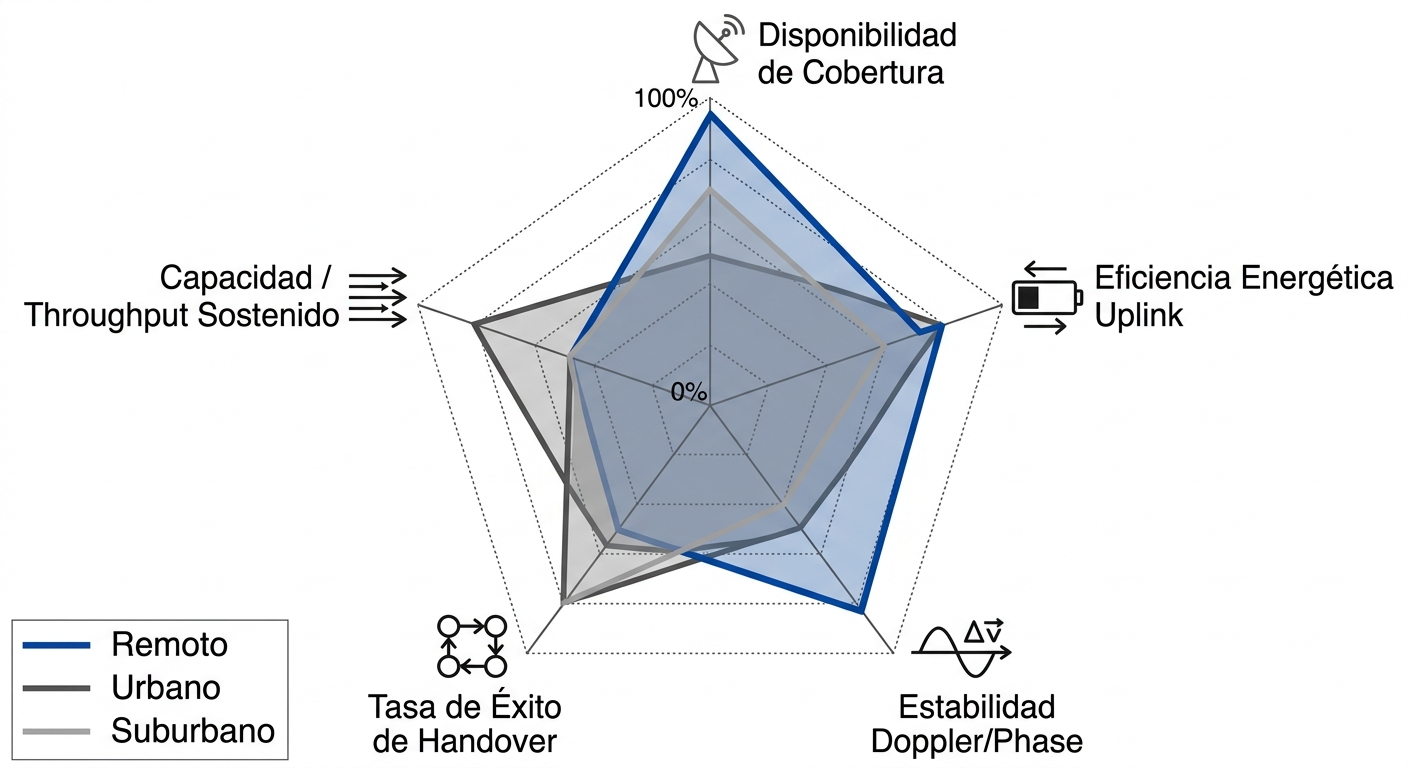
\includegraphics[width=0.95\linewidth]{fig5.png}
\scalebox{0.5}{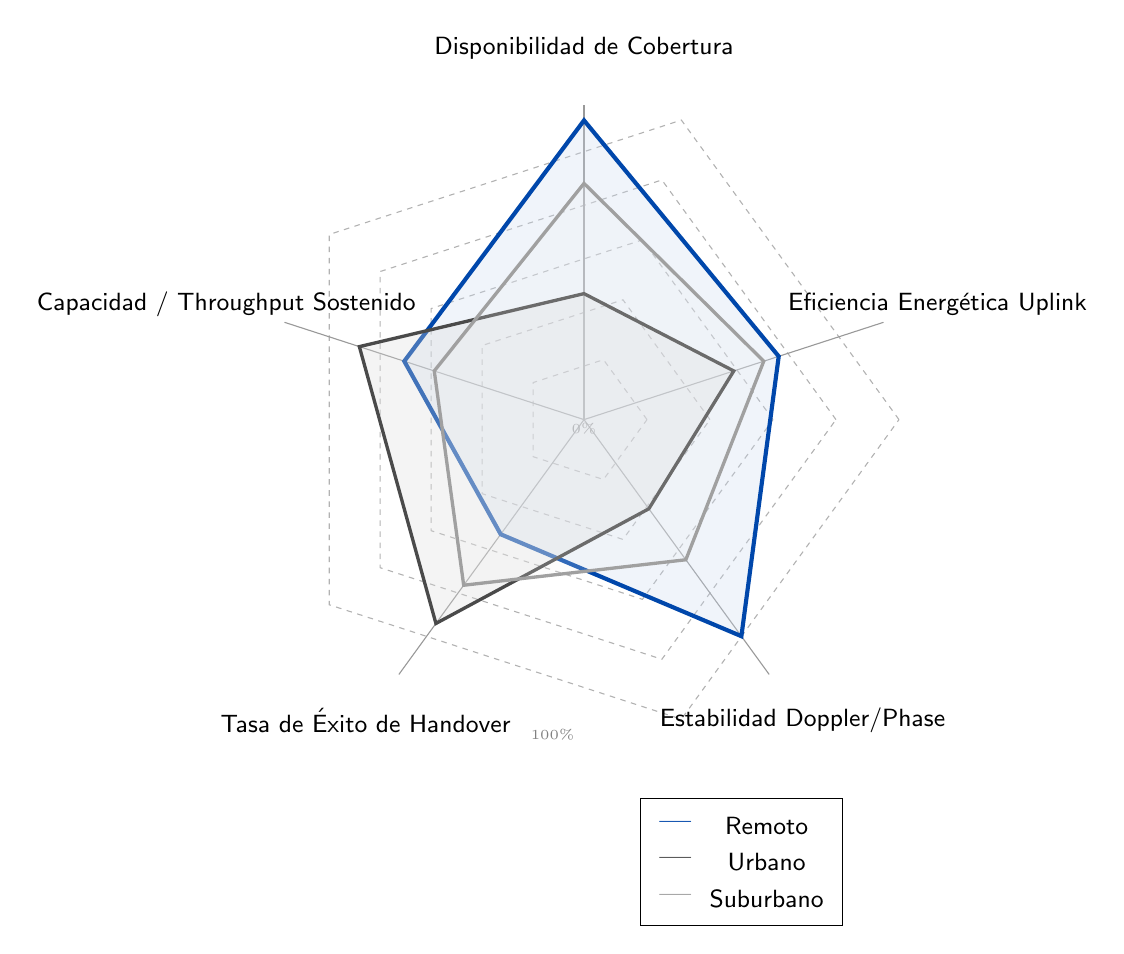
\begin{tikzpicture}[scale=4, font=\sffamily\small]
    % --- Definición Moderna de Estilos ---
    \tikzset{
        gridline/.style={dash pattern=on 2pt off 2pt, color=gray!60, thin},
        axisline/.style={color=black!40, thin}
    }
    
    % --- Dibujo de la Red Concéntrica (Grid Pentagonal) ---
    \foreach \r in {0.2, 0.4, 0.6, 0.8, 1.0} {
        \draw[gridline] (0:\r) -- (72:\r) -- (144:\r) -- (216:\r) -- (288:\r) -- cycle;
    }
    
    % --- Ejes Radiales y Etiquetas (Corregido sin la clave 'digital') ---
    \foreach \a/\label in {
        90/{Disponibilidad de Cobertura},
        18/{Eficiencia Energética Uplink},
        306/{Estabilidad Doppler/Phase},
        234/{Tasa de Éxito de Handover},
        162/{Capacidad / Throughput Sostenido}
    } {
        \draw[axisline] (0,0) -- (\a:1.0);
        \node[align=center] at (\a:1.18) {\label};
    }
    
    % Etiquetas de escala de porcentaje interno
    \node[below, gray, font=\tiny] at (90:0.02) {0\%};
    \node[left, gray, font=\tiny] at (270:1.0) {100\%};

    % --- POLÍGONO 1: REMOTO (Azul Cobalto) ---
    \definecolor{remotoblue}{HTML}{0047AB}
    \draw[color=remotoblue, line width=1.5pt, fill=remotoblue!20, fill opacity=0.3] 
        (90:0.95) -- (18:0.65) -- (306:0.85) -- (234:0.45) -- (162:0.60) -- cycle;

    % --- POLÍGONO 2: URBANO (Gris Oscuro) ---
    \definecolor{urbanogray}{HTML}{4A4A4A}
    \draw[color=urbanogray, line width=1.2pt, fill=urbanogray!20, fill opacity=0.3] 
        (90:0.40) -- (18:0.50) -- (306:0.35) -- (234:0.80) -- (162:0.75) -- cycle;

    % --- POLÍGONO 3: SUBURBANO (Gris Claro) ---
    \definecolor{suburbanogray}{HTML}{A0A0A0}
    \draw[color=suburbanogray, line width=1.2pt, fill=suburbanogray!15, fill opacity=0.2] 
        (90:0.75) -- (18:0.60) -- (306:0.55) -- (234:0.65) -- (162:0.50) -- cycle;
        
    % --- Leyenda de los Escenarios ---
    \matrix [draw, fill=white, at={(0.5,-1.2)}, anchor=north] {
        \node [color=remotoblue, font=\bfseries] {---}; & \node {Remoto}; \\
        \node [color=urbanogray, font=\bfseries] {---}; & \node {Urbano}; \\
        \node [color=suburbanogray, font=\bfseries] {---}; & \node {Suburbano}; \\
    };
\end{tikzpicture}}
\caption{Análisis de cobertura simulada para conectividad D2D-NTN en escenarios urbanos, suburbanos y remotos.}
\label{fig:coverage_analysis}
\end{figure}

La Tabla 4 sintetiza los principales trade-offs. Aunque los resultados de simulación son prometedores, persisten limitaciones importantes en escenarios de alta densidad de dispositivos, lo que señala la necesidad de continuar investigando técnicas de agrupamiento cooperativo y transmisión discontinua.